\documentclass[a4paper,12pt]{article}

\usepackage{amssymb,amsmath}
\usepackage[brazilian]{babel}
\usepackage[utf8]{inputenc}
\usepackage{graphicx}
\usepackage{chngcntr}
\usepackage{tikz}
\usepackage{tikz-3dplot}
\usepackage{indentfirst}
\usepackage[numbers,sort&compress]{natbib}
\usepackage[title]{appendix}
\usepackage{subfig}
\usepackage{floatrow}
\usepackage{booktabs}% http://ctan.org/pkg/booktabs
\newcommand{\tabitem}{~~\llap{\textbullet}~~}

\usetikzlibrary{trees}
\usetikzlibrary{decorations.pathmorphing}
\usetikzlibrary{decorations.markings}

\tikzset{
    photon/.style={decorate, decoration={snake}, draw=black},
    fermion/.style={draw=black, postaction={decorate}, 
    decoration={markings,mark=at position .55 with {\arrow[scale=2,draw=black]{>}}}},
    afermion/.style={draw=black, postaction={decorate}, 
    decoration={markings,mark=at position .55 with {\arrow[scale=2,draw=black]{<}}}},
    gluon/.style={decorate, draw=green,
    decoration={coil,amplitude=4pt, segment length=5pt}} 
    }

\counterwithin{figure}{subsection}

\usepackage{afterpage}

\newcommand\blankpage{%
    \null
    \thispagestyle{empty}%
    \addtocounter{page}{-1}%
    \newpage}
    
\setlength{\parindent}{20pt}


\renewcommand{\and}{\\}
%opening
\title{Estudo de subestrutura de jatos de quarks pesados em colisões de íons pesados}
\author{Fabio de Moraes Canedo
\and Marcelo Gameiro Munhoz}

\begin{document}

\maketitle

\begin{abstract}
A proposta descrita nesse projeto é a de realizar estudos a respeito da fase da matéria conhecida
como plasma de quarks e gluons(\emph{quark-gluon plasma}-QGP) através de observáveis que se relacionam
com quarks pesados(\emph{charm} e \emph{beauty}). Os observáveis visados nesse trabalho referem-se
à estrutura interna de jatos pesados. Especificamente, testaremos modelos diferentes para a geração
de eventos e estudaremos funções de fragmentação através da distribuição angular e energética de subjatos.
\end{abstract}

%%Arquivo teste para imagens

\begin{figure}
 \begin{center}
 %\tdplotsetmaincoords{70}{120}
 %[tdplot_main_coords, scale=1]

 \begin{tikzpicture}[
        thick,
        % Set the overall layout of the tree
        level/.style={level distance=1.5cm},
        level 2/.style={sibling distance=2.6cm},
        level 3/.style={sibling distance=2cm}
    ]
    \coordinate
        child[grow=left, level distance=0pt]{
            child {
                node {$g$}
                % The 'edge from parent' is actually not needed because it is
                % implicitly added.
                edge from parent [gluon]
            }
            child {
                node {$g$}
                edge from parent [gluon]
            }
        }
        % I have to insert a dummy child to get the tree to grow
        % correctly to the right.
        child[grow=right, level distance=0pt]{
	  child {
	    node {$g$}
	      edge from parent [gluon]
	  }
	  child {
	  node {$g$}
										edge from parent [gluon]
		}
								};
						\end{tikzpicture}

\caption{Tikzpicture}
\label{Tikzpicture}

 \end{center}

\end{figure}

\section{Introdução}

\subsection{Plasma de Quarks e Gluons}
Em colisões íons pesados(íons de chumbo ou ouro) a uma energia da ordem de $100 GeV$,
como na Figura \ref{qgp},é possível realizar a quebra momentânea dos hádrons constituintes desses núcleos, liberando novos graus
de liberdade para o movimento dos quarks, dessa maneira, atinge-se um novo estado da matéria, chamado Plasma de Quarks e Gluons,
ou QGP\footnote{Sigla em inglês para Plasma de Quarks e Gluons}. A temperatura necessária para formar este estado da matéria é da
ordem de milhares de $MeV$ ou $10^{10} K$, e a densidade de energia é da ordem de $0.2-1 GeV/fm^{3}$. As propriedades deste estado
da matéria podem ser estudadas analisando os produtos dessa colisão após o resfriamento da matéria. Através espectro de
$p_T$\footnote{Ver Apêndice \ref{variaveis}} das partículas, por exemplo, fornece insformações sobre a entropia e a temperatura do
plasma, através da multiplicidade e da inclinação do gráfico, respectivamente. Em geral, essas propriedades, referentes à expansão
hidrodinâmica do plasma\footnote{Ver Apêndice \ref{hidrodinamica}} estarão associados ao espectro na faixa de $p_T \approx 0-2 GeV/c$.
Na faixa $p_T > 2 GeV/c$, observa-se os efeitos de fenômenos da classe {\it hard scaterring}. Essas propriedadess são resultados da formação
de partículas de alta energia que atravessam o plasma aquecido, depositando energia neste. Na sua saída, devido às propriedades\footnote{Para
mais detalhes sobre as propriedades citadas, ver \cite{skands_introduction_2013}} da QCD\footnote{QCD ou {\it Quantum Chromodynamics}
é a teoria que descreve as interações fortes.}, essas partículas se fragmentam criando os chamados jatos ou {\it jets}\footnote{Para
uma definição mais precisa de jatos, ver Apêndice \ref{algoritmos}}. Esses jatos sofrem efeitos estruturais por conta da interação dos
partons iniciais\cite{lokhtin_angular_1998,bass_systematic_2009,connors_review_2017,nattrass_jet_2018,denterria_jet_2009} com o plasma.

%\begin{figure}[!h]


 \centering
 \begin{tikzpicture}[thick,scale=.3]

\fill[red] (0,23) ellipse (2 and 3) node [black,scale=1] {Pb};

\fill[red] (8,21) ellipse (2 and 3) node [black,scale=1] {Pb};

\shade[outer color=red,inner color=orange] (3,13) ellipse (2 and 3) -- (5,11) ellipse (2 and 3);

\shade[inner color=yellow, outer color=red,decorate,decoration={snake,amplitude=3,segment length=20}] (4,1.5) circle (3) node [scale=1] {QGP};

\end{tikzpicture}
\caption{Sequência temporal de colisão de íons pesados.}
\label{qgp}
\end{figure}

\begin{figure}[!h]
 \centering
 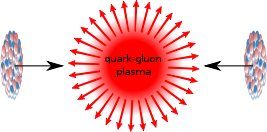
\includegraphics[scale=1]{Content/qgp.png}
 \caption{Colisão de núclos pesados, resultando na formação do Plasma de Quarks e Gluons.}
 \label{qgp}
\end{figure}


Assim como a perda de energia de jatos, ou \emph{jet quenching}, outros efeitos são considerados como assinaturas do Plasma de Quarks e Gluons,
tal como o aumento da produção de estranheza e a supressão de produção do $J/\Psi$ em relação às colisões $pp$. A produção de estranheza é uma assinatura que provém do
equilíbrio químico(ver \cite{letessier_hadrons_2002}) supostamente gerado no início da colisão. Esse aumento da produção de estranheza, ou \emph{strange production enhancement},
foi observado, em comparação com colisões p-p ou p-Pb, e pode ser observado na Figura \ref{strangeness}.

\begin{figure}
 \centering
 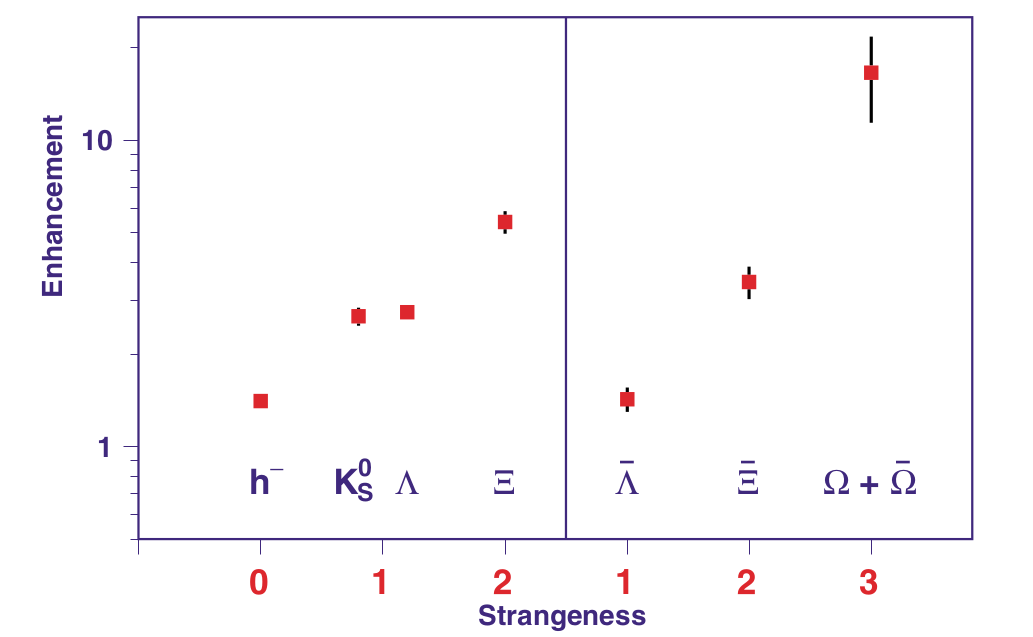
\includegraphics[scale=.3]{Content/strangeness.png}
 \caption{Aumento da produção de estranheza. O aumento é definido pela razão entre o número de contagens em colisões Pb-Pb e as contagens em p-Be. Resultados obtidos pelo experimento
 CERN WA97.}
 \label{strangeness}
\end{figure}

\subsection{Quarks Pesados como Ponta de Prova}
No início de colisões de íons pesados, quarks pesados podem ser gerados através dos mecanismos mostrados na Figura \ref{criacao}.

\begin{figure}[!hbt]
\begin{floatrow}
 \subfloat[Criação de par através de aniquilação de gluons.]{
 \begin{tikzpicture}[scale=.45]
  \draw [gluon] (0,3) -- (4,2.5) node[near start,anchor=south,red]{$g$};
  \draw [gluon] (0,0) -- (4,.5) node[near start,anchor=north,red]{$g$};
  \draw [afermion] (4,2.5) -- (8,3) node[near end,anchor=south,red]{$\overline{Q}$};
  \draw [fermion] (4,2.5) -- (4,.5);
  \draw [fermion] (4,.5) -- (8,0) node[near end,anchor=south,red]{$Q$};
 \end{tikzpicture}
 \label{diagramaa}
 }
 
 \subfloat[Criação de par de quarks pesados através de aniquilação de quarks leves oriundos dos núcleons iniciais.]{
 \begin{tikzpicture}[scale=.35]
  \draw [fermion] (0,4) -- (3,2) node[near start,anchor=south,red]{$q$};
  \draw [afermion] (0,0) -- (3,2) node[near start,anchor=north,red]{$\overline{q}$};
  \draw [gluon] (3,2) -- (5,2);
  \draw [fermion] (5,2) -- (8,4) node[near end,anchor=south,red]{$Q$};
  \draw [afermion] (5,2) -- (8,0) node[near end,anchor=north,red]{$\overline{Q}$};
 \end{tikzpicture}
 \label{diagramab}
 }
 
 \subfloat[Mesmo processo do caso anterior, mas com emissão de gluon posterior.]{
 \begin{tikzpicture}[scale=.45]
  \draw [gluon] (0,3) -- (4,2.5) node[near start,anchor=south,red]{$g$};
  \draw [gluon] (0,0) -- (4,.5) node[near start,anchor=north,red]{$g$};
  \draw [afermion] (4,2.5) -- (8,3) node[near end,anchor=south,red]{$\overline{Q}$};
  \draw [fermion] (4,2.5) -- (4,.5);
  \draw [fermion] (4,.5) -- (8,0) node[near end,anchor=north,red]{$Q$};
  \draw [gluon] (5,.375) -- (8,1.5) node[near end,anchor=south,red]{$g$};
 \end{tikzpicture}
 \label{diagramac}
 }
 
 \end{floatrow}
 
 \begin{floatrow}
  \subfloat[]{
 \begin{tikzpicture}[scale=.45]
  \draw [gluon] (0,3) -- (4,2.5) node[near start,anchor=south,red]{$g$};
  \draw [fermion] (4,2.5) -- (8,3) node[near end,anchor=south,red]{$Q$};
  \draw [afermion] (4,2.5) -- (5,2);
  \draw [gluon] (0,0) -- (4,0) node[near start,anchor=north,red]{$g$};
  \draw [gluon] (4,0) -- (5,2);
  \draw [gluon] (4,0) -- (8,0) node[near end,anchor=north,red]{$g$};
  \draw [afermion] (5,2) -- (8,2) node[near end,anchor=north,red]{$\overline{Q}$};
 \end{tikzpicture}
 }
 
 \subfloat[]{
 \begin{tikzpicture}[scale=.45]
  \draw [gluon] (0,3) -- (3,2.5) node[near start,anchor=south,red]{$g$};
  \draw [gluon] (3,2.5) -- (5,2.5);
  \draw [gluon] (0,0) -- (3,0)node[near start,anchor=north,red]{$g$};
  \draw [gluon] (3,0) -- (3,2.5);
  \draw [gluon] (3,0) -- (8,0) node[near end,anchor=north,red]{$g$};
  \draw [afermion] (5,2.5) -- (8,2) node[near end,anchor=north,red]{$\overline{Q}$};
  \draw [fermion] (5,2.5) -- (8,3) node[near end,anchor=south,red]{$Q$};
 \end{tikzpicture}
 }
 
 \subfloat[]{
 \begin{tikzpicture}[scale=.45]
  \draw [gluon] (0,4.5) -- (2,3.5) node[near start,anchor=south,red]{$g$};
  \draw [afermion] (2,3.5) -- (8,6.5) node[near end,anchor=south,red]{$\overline{Q}$};
  \draw [fermion] (2,3.5) -- (3,2.5);
  \draw [fermion] (3,2.5) -- (8,4.5) node[near end,anchor=south,red]{$Q$};
  \draw [gluon] (3,2.5) -- (4,1.5);
  \draw [gluon] (4,1.5) -- (8,3.5) node[near end,anchor=north,red]{$g$};
  \draw [gluon] (4,1.5) -- (4,0);
  \draw [gluon] (0,0) -- (4,0) node[near start,anchor=north,red]{$g$};
  \draw [gluon] (4,0) -- (8,0) node[near end,anchor=north,red]{$g$};
 \end{tikzpicture}
 }
 
 \end{floatrow}

 
 \caption{Processos de criação de quarks pesados.}
 \label{criacao}
\end{figure}


Quarks pesados, como o \emph{bottom}, podem ser utilizados como ponta de prova para o estudo do Plasma de Quarks e Gluons
devido à sua interação com o este em seu caminho para fora da região de interação\cite{li_inverting_2017,renk_jet_2014}. Eles
interagem com o meio de duas formas, através da radiação induzida, ou \emph{gluonsstrahlung}, e através de reações colisionais.
Embora estes mesmos feitos ocorram para quarks leves, a massa dos quarks pesados limita a sua perda de energia e também sua
velocidade\footnote{Especialmente no limite $E \approx m$}, o que permite que ele ``colete'' mais informações sobre o QGP.
\par
Os efeitos do meio podem ser especialmente observados na subestrutura dos jatos, que são causadas por funções de fragmentação.
Estas, por sua vez, estão diretamente relacionadas com os processos de perda de energia do parton no QGP. As funções de fragmentação
são distribuições de probabilidade que refletem processos do tipo $a \longrightarrow b+c$. Para um certo número $z \in [0,1]$, teremos
a relação entre as energias:

\begin{equation}
 E_a = z E_b + (1-z)E_c
\end{equation}

Podemos então, definir a função densidade de probabilidade do processo:

\begin{equation}
 P_{a \longrightarrow b+c}(z) = \frac{dN_{a \longrightarrow b+c}}{dz}
 \label{probz}
\end{equation}

Essa função pode ser medida na subestrutura dos jatos, assim como a equivalente em abertura angular:

\begin{equation}
 P_{a \longrightarrow b+c}(\theta) = \frac{dN_{a \longrightarrow b+c}}{d\theta}
 \label{probt}
\end{equation}

Essas quantidades podem ser calculadas com a utilização da pQCD\footnote{\emph{perturbative Quantum Chromodynamics}}, um exemplo desses
cálculos pode ser encontrado em \cite{seymour_jet_1998}. Esses efeitos, como supramencionado, podem ser observados na subestrutura dos
jatos. Por sua vez, a subestrutura pode ser observada através de variações no parâmetro $R$ nos algoritmos de reconstrução de jatos(ver
Apêndice \ref{algoritmos}. Ao diminuirmos esse parâmetro, os algoritmos evitam o \emph{merge} dos jatos e podemos então, para dois
jatos próximos comparar o a distância angular de dois jatos($\Delta R$) e a fração de energia que o jato mais leve possui da soma total.
Isso deve fornecer evidência direta das funções de probabilidade definidas nas equações \eqref{probz} e \eqref{probt}.

\newpage

\section{Objetivo}
A intenção do trabalho é a realização de simulações para analisar certos observáveis para o estudo de quarks pesados
com objetivo de extrair informações do QGP, através de mecanismos supracitados. Especificamente,
iremos verificar a relação entre modelos de perda de energia e os observáveis de subestrutura
de jatos. Os observáveis estudados serão a distância angular entre os centro dos subjatos e 
a fração energética compartilhada entre ambos. Certos modelos \cite{zapp_monte_2009, renk_jet_2014} preveem
que o meio deve interferir em processos de perda de energia através de processos como os da Figura \ref{proc_perd}.

\begin{figure}[!htb]
\begin{floatrow}

\subfloat[Colisão elástica com gluons do meio.]{
 \begin{tikzpicture}[scale=.5]
 \draw [fermion] (0,4) -- (2,2);
 \draw [gluon] (0,0) -- (2,2);
 \draw [fermion] (2,2) -- (4,2);
 \draw [gluon] (4,2) -- (6,0);
 \draw [fermion] (4,2) -- (6,4) node[anchor=south,red]{$Q$};
 \end{tikzpicture}
 }
 
 \subfloat[Radiação induzida pelo meio.]{
 \begin{tikzpicture}[scale=.5]
  \draw [fermion] (0,4) -- (2,2);
 \draw [gluon] (0,0) -- (2,2);
 \draw [fermion] (2,2) -- (4,2);
 \draw [gluon] (5,3) -- (7,3);
 \draw [gluon] (4,2) -- (6,0);
 \draw [fermion] (4,2) -- (6,4) node[anchor=south,red]{$Q$};
 \end{tikzpicture}
 
 }
 
\end{floatrow}

\caption{Processos de perda de energia no meio}
\label{proc_perd}

\end{figure}

Em ambos os casos descritos na Figura \ref{proc_perd}, a perda de energia é afetada por elementos de matriz que carregam
informações do meio, especialmente nos gluons iniciais da colisão. Portanto, o meio afeta as fragmentações e deve afetar
as subestruturas finais dos jatos. Assim um jato $p_\mu$ que pode ser quebrado em dois subjatos $p_{1\mu}$ e $p_{2\mu}$,
tal que $p_\mu=p_{1\mu}+p_{2\mu}$, pode ser analizado através dos números $z$ e $R_{12}$ nas equações:

\begin{equation}
 \begin{split}
  E &= zE_1 + (1-z) E_2 \\
  R_{12} &= sqrt{ (y_1-y_2)^2 + (\phi_1-\phi_2)^2 }
 \end{split}
\end{equation}

Podemos então analisar a função $\frac{dN}{dz}$ e $\frac{dN}{dR_{12}}$ e formar espectros que, posteriormente, podem ser
comparados para os casos de colisões $pp$.

\newpage

\section{Plano de Trabalho e Cronograma}
Abaixo, segue o cronograma planejado para a realização do trabalho:

\begin{tabular}{|c|p{8cm}|}
  \hline
  1º semestre de 2018 & Obtenção dos créditos do programa de pós-graduação do IFUSP \\
		      & Estudos introdutórios da área de íons pesados relativísticos \\ \hline
  2º semestre de 2018 & Obtenção dos créditos do programa de pós-graduação do IFUSP \\
		      & Estudo e contextualização do problema a ser investigado: \\
		      & \tabitem Levantamento bibliográfico sobre os processos de produção de quarks pesados; \\
		      & \tabitem Estudo de alguns geradores de evento de colisões hadrônicas, com ênfase nos processos de perda de energia dos quarks pesados; \\
		      & \tabitem Estudo dos algoritmos de reconstrução de jatos, bem como dos algoritmos que podem realizar análise de subestrutura dos jatos. \\ \hline
  1º semestre de 2019 & Simulação de eventos com os modelos e geradores estudados previamente \\
  		      & Início da análise dos dados \\ \hline
  2º semestre de 2019 & Finalização da análise dos dados simulados \\
  		      & Redação da dissertação \\ \hline
\end{tabular}


\newpage

\section{Material e Métodos}
Para a realização desse trabalho utilizaremos geradores de eventos, que são essencialmente simuladores
de colisões de íons pesados, para verificar os efeitos esperados das fragmentações de quarks pesados
nos observáveis de subestrutura de jatos. Os programas que serão utilizados serão:

\begin{itemize}
 \item MUSIC\cite{noauthor_music_nodate}, que possui uma breve descrição na subseção \ref{music};
 \item PYTHIA\cite{noauthor_pythia_nodate}, que constitui em um gerador de jatos, especificamente;
 \item HYDJET\cite{lokhtin_hydjet++_2009}, constitui um gerador de jatos combinado com um algoritmo de simulação hidrodinâmica, ver subseção \ref{hjet};
 \item Jewel\cite{noauthor_jewel_nodate, zapp_jewel_2014}, constitui um gerador de eventos com modelos específicos de \emph{Jet Quenching};
\end{itemize}


\subsection{MUSIC}\label{music}
O programa MUSIC, a ser utilizado nas simulações deste trabalho, é um
gerador de eventos que pode ser encontrado em \cite{noauthor_music_nodate}.
\par
Em \cite{schenke_3+1d_2010} encontramos uma descrião mais detalhada do algoritmo empregado. Alguns fatos
são citados a seguir:

\begin{itemize}
 \item O método KURGANOV-TADMOR é implementado, este método baseia-se na introdução de
 um termo de dissipação numérica para garantia de estabilidade, é capaz de lidar com
 choques e descontinuidades, ideal para a inserção de termos fonte como deposição de energia
 de jatos;
 \item As condições iniciais são baseadas no modelo de Glauber e na parametrização de Woods-Saxon,
 ver subseção \ref{glauber};
 \item Uma simplificação das equações é atingida escolhendo variáveis através de uma rotação hiperbólica;
 \item O {\it freeze-out} é construído assumindo a fórmula de Cooper-Frye\cite{teaney_chemical_2002};
\end{itemize}

É interessante observar na Figura \ref{fig:musicv2} que o MUSIC não fornece resultados coerentes com os experimentos na faixa de $p_T$
entre $1$ e $2 GeV$. Isso poderia ser explicado pela ausência de energia depositada pelos jatos, que incluem na hidrodinâmica efeitos
anisotrópicos\cite{andrade_jet_2014}, ver Figura \ref{fig:v2}.

\begin{figure}[!h]
\centering
 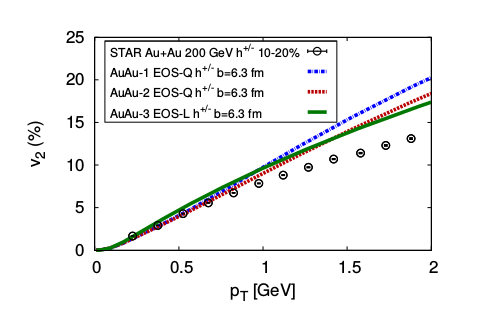
\includegraphics[scale=0.5]{Content/music_results.png}
 \caption{Resultados do MUSIC no coeficiente $V_{2}$.}
 \label{fig:musicv2}
\end{figure}


\subsection{HYDJET++}\label{hjet}
O gerador de eventos HYDJET++, descrito em \cite{lokhtin_hydjet++_2009} trabalha com dois
processos distintos para a geração de eventos nas partes {\it hard} e {\it soft} das
colisões de íons pesados.
\par
O processo {\it hard} se dá através de um modelo de perda de energia baseado na equação:

\begin{equation}
 \Delta E (L, E) = \int_{0}^{L} dl \frac{dP(l)}{dl} \lambda (l) \frac{dE(l,E}{dl},
 \frac{dP(l)}{dl} = \frac{1}{\lambda (l)} \exp{-l/\lambda (l)}
\end{equation}

Nesta equação, temos um termo $\frac{dP(l)}{dl}$ como a probabilidade de \emph{scattering} no meio
por unidade de comprimento atravessado pelo parton, $\lambda (l)$ é o livre caminho médio, e
$\frac{dE(l,E}{dl}$ descreve a perda de energia por unidade de comprimento atravessado. Neste último
termo, reações colisionais e radiativas são levadas em consideração. O espectro final, assim como o
formato angular da emissão é calculado utilizando o gerador PYQUEN\cite{noauthor_pyquen_nodate}, que é uma versão modificada
do PYTHIA\cite{noauthor_pythia_nodate}. Os \emph{partons} são gerados de acordo com o algoritmo PYTHIA, então, são
feitos os espalhamentos respectivos durante seu caminho pelo QGP e também sua emissão radiativa. Em seguida,
a hadronização é realizada através de um modelo de Lund\cite{skands_introduction_2013} para os \emph{partons} de alta energia e
também para os \emph{gluons} de alta energia emitidos.

\par

A parte \emph{soft} do algoritmo é implementada através de implementação numérica tridimensional hidrodinâmica
com uma superfície de freeze-out que emite partículas conforme a distribuição:

\begin{equation}
 f_{i}^{eq} (p^{*0} ;T^{ch} ,\mu_i , \gamma_s) = \frac{ g_i }{ \gamma_s^{-n_{i}^{s}} \exp{ ( [p^{*0} - \mu_i]/T^{ch} ) } \pm 1 }
\end{equation}

Esta distribuição representa um corpo negro emitindo as partículas à temperatura $T^{ch}$. A energia das partículas é calculada
no referencial de repouso da superfície e é representada por $p^{*0}$. $\mu_i$ representa o potencial químico das partículas e
$\gamma_s$ é o fator de supressão de estranheza.

\newpage

\section{Análise dos Dados}
A análise dos dados será feita através de programas de \emph{jet clustering}, especificamente
o FastJet\cite{noauthor_fastjet_nodate}. As funções de distribuição de energia e ângulo serão
calculadas para uma série de eventos. Os algoritmos que são utilizados nesse programa são descrito
no Apêndice \ref{algoritmos}. Com o uso desses algoritmos, a análise será feita previamente localizando
os jatos nos dados. Em seguida, variando parâmetros como o $R$ ou parando em passos anteriores como no
caso do algoritmo $k_T$, podemos identificar subjatos dentro dos jatos. Após esse procedimento, é possível
medir abertura angular e fração energética dos jatos. Os histogramas montados para cada modelo
irão apresentar o comportamento dos observáveis em cada caso.

\begin{appendices}

\section{Algoritmos de \emph{Jet Clustering}}\label{algoritmos}
Para se estudar jatos, é necessário definir uma maneira de agrupar as partículas medidas nos detectores 
de uma maneira coerente e bem definida, como os requisitos do \emph{Snowmass accord}:

\begin{enumerate}
 \item Simples de implementar em uma análise experimental;
 \item Simples de implementar em um cálculo teórico;
 \item Definido em todas as ordens em cálculos perturbativos;
 \item Gera seções de choque finitas em todas as ordens;
 \item É insensível à hadronização;
\end{enumerate}

Para realizar a reconstrução de jatos\cite{salam_towards_2010}, costuma-se definir a seguinte quantidade:

\begin{equation}
 \Delta R_{ij} = \sqrt{(\eta_i-\eta_j)^2+(\phi_i-\phi_j)^2}
\end{equation}

Essa será, para as duas partículas, aqui chamadas de $i$ e $j$, uma distância angular
definida entre as duas. A maioria dos algoritmos de jatos irão utilizar essa definição de distância angular para realizar os agrupamentos,
ou {\it clusters} de partículas para a reconstrução dos jatos. Estes são chamados os algoritmos de cones. Um algoritmo
comumente utilizado consiste em, primeiro definir um parâmetro $R$, em seguida, escolher uma partícula {\it semente}, normalmente, escolhe-se
a partícula de maor $p_T$. Após esses passos, localizamos a partícula de maior $p_T$ a uma distância menor ou igual a $R$.
\par
Então, retiramos essas duas partículas dos dados e definimos uma nova partícula com momento:

\begin{equation}
 p_{\mu}^{J} = p_{\mu}^1 + p_{\mu}^2
\end{equation}

Essa partícula define o novo centro do cone, agora procuramos a partícula de maior $p_T$ de distância menor ou igual a $R$ desta, e assim por
diante. Os métodos de reconstrução de jatos todos irão seguir alguma rotina que envolva calcular distâncias entre os hadrons de acordo com
alguma métrica que utiliza a metida invariante acima, como eles podem precoder a partir daí varia, alguns exemplos são citados:

\begin{description}
 \item[IC-PR] são os algoritmos de cones interativos de remossão progressiva, isso
 quer dizer que eles mudam a direção do cone a cada interação e retiram os jatos um de
 cada vez;
 \item[FC-PR] são semelhantes aos {\bf IC-PR}, mas as direções dos cones são fixas ao redor
 da semente;
 \item[IC-SM] são os algoritmos que utilizam cones iterativos, mas não removem os cones
 estáveis, para lidar com \emph{overlapping}, utiliza-se métodos que envolvem atribuir cada
 partícula ao jato mais próximo ou simplesmente juntar os dois jatos, baseando-se na fração
 da quantidade de energia que o jato menos intenso que está na região de \emph{overlapping};
 \item[IC-SD] aplicam o \emph{split and drop}, ou seja, ele não une jatos que dividem muita
 energia em comum, mas simplesmente desconsideram os jatos menos intensos;
 \item[SR] são uma classe de algoritmos que combinam partículas({\it Sequential Recombination}) em jatos baseando-se
 em uma metrica pŕe-definida, que é o caso do {\it $k_T$ algorithm};
\end{description}




\section{Variáveis}\label{variaveis}
\subsection{Rapidity}

Uma variável útil de se definir em um estudo de colisões de partículas a velocidades relativísticas é a {\it rapidity} $y$. Mas antes,
definimos o conceito de massa transversa.
\par
Toda colisão de partículas possui um eixo específico, chamdo eixo de colisão. Associado a este eixo, há um plano transverso. As componentes
dos momentos no eixo da colisão e no plano transverso serão identificadas como $p_{L}$ e $p_{T}$, respectivamente. Essas variáveis podem ser
melhor compreendidas observando a Figura \ref{fig:geometria}.

\begin{figure}[!h]
 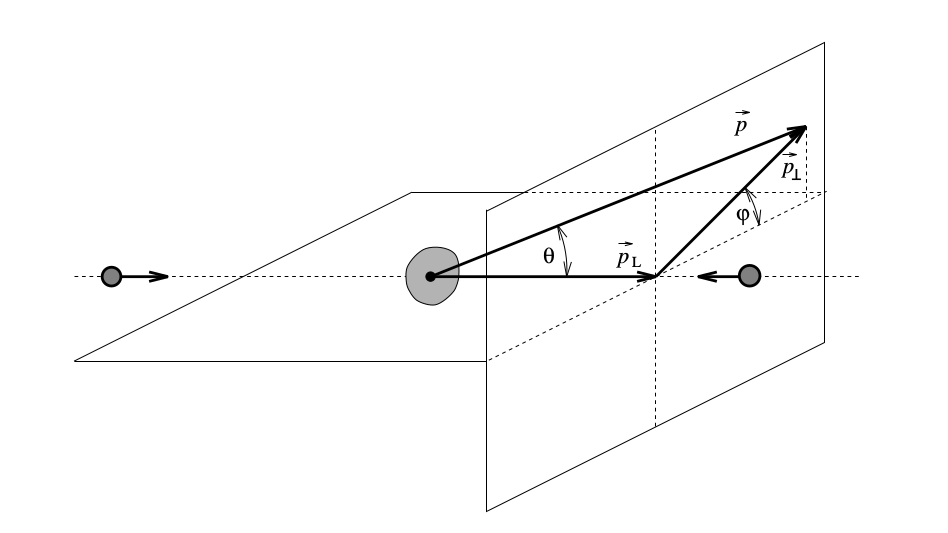
\includegraphics[scale=0.35]{Content/geometriamomento.png}
 \caption{Ilustração geométrica de $p_T$ e $p_L$.}
 \label{fig:geometria}
\end{figure}


Associada ao momento transversal, definimos a massa transversa:

\begin{equation}
 m_{T}=\sqrt{m^2+p_{T}^2}
\end{equation}

Ao contrário de $p_{L}$, $p_{T}$ não depende do referencial em que a colisão é estudada, portando, é uma boa variável. É necessário, então,
definir uma variável no eixo de colisão, esta será a {\it rapidity}. Definimos esta através das equações:

\begin{subequations}
\begin{align}
 E=m_{T} \cosh{(y)} \\ p_{L}=m_{T} \sinh{(y)}
\end{align}
\end{subequations}

Isolando $\eta$ nas equações acima obtemos:

\begin{equation}
 y = \ln{(\frac{E+p_{L}}{m_{T}})}
\end{equation}

Uma propriedade importante desta variável, é que ela é aditiva em relação a transformações de Lorentz.

\subsection{Pseudorapidity}

Quando a energia de uma partícula é muito grande comparada à sua massa, podemos escrever:

\begin{equation}
\begin{split}
 y   & = \ln{\frac{E+p_{L}}{m_{T}}} \\
     & = \frac{1}{2}\ln{\frac{(E+p_{L})^2}{m_{T}^2}} \\
     & = \frac{1}{2}\ln{\frac{(E+p_{L})^2}{E^2-p_{L}^2}} \\
     & = \frac{1}{2}\ln{\frac{E+p_{L}}{E-p_{L}}} \\
     & \approx \frac{1}{2}\ln{\frac{p+p_{L}}{p-p_{L}}} \\
     & \approx \frac{1}{2}\ln{\frac{1+\cos(\theta)}{1-\cos(\theta)}} \\
     & \approx \frac{1}{2}\ln{\cot{2\theta}} \\
\end{split}
\end{equation}

Definimos então, a variável {\it pseudorapidity}:

\begin{equation}
 \eta = \frac{1}{2}\ln{\cot{2\theta}}
\end{equation}



\section{Hidrodinâmica Relativística}\label{hidrodinamica}
Para descrever a evoluão do QGP, utiliza-se o formalismo da hidrodinâmica relativística. Algumas quantidades são
importantes de serem definidas:

\begin{equation}
 \frac{dx^{\mu}}{d\tau} = u^{\mu}(x)
\end{equation}

Essa será a velocidade, ou fluxo do fluido em cada elemento do espao-tempo. Também teremos o tensor energia-momento:

\begin{equation}
 T_{\mu \nu} = (\epsilon + P) u_\mu u_\nu - P g_{\mu \nu}
\end{equation}

Se aplicarmos a equação de conservação de energia-momento, obtemos quatro equações que descrevem a evoluao do fluido:

\begin{equation}
 \partial^\mu T_{\mu \nu} = 0
\end{equation}

Entretanto, temos quatro variáveis $u^{\mu}$ e mais duas $\epsilon$ e $P$, totalizando seis. Para resolvermos o sistema precisamos
de duas equações adicionais, são estas a normalização do quadrivetor($u^{\mu}u_{\mu}=1$ e a equação de estado:

\begin{equation}
 \epsilon=\epsilon(P)
\end{equation}




\section{Modelo de Lund}
A teoria que descreve as interações mediadas por \emph{gluons} é a
QCD\footnote{Sigla em inglês para Cromodinâmica Quântica}. É uma teoria
de calibre não-abeliana, o que significa que os bósons mediadores
de suas interações podem interagir entre si também, formando vértices
constituídos apenas por \emph{gluons}, como na Figura \ref{fourgluon}.

	\usetikzlibrary{trees}
	\usetikzlibrary{decorations.pathmorphing}
	\usetikzlibrary{decorations.markings}
	
	\tikzset{
				    photon/.style={decorate, decoration={snake}, draw=red},
				    electron/.style={draw=blue, postaction={decorate},
				        decoration={markings,mark=at position .55 with {\arrow[draw=blue]{>}}}},
				    gluon/.style={decorate, draw=magenta,
				        decoration={coil,amplitude=4pt, segment length=5pt}} 
				}
				
	\begin{tikzpicture}[
				        thick,
				        % Set the overall layout of the tree
				        level/.style={level distance=1.5cm},
				        level 2/.style={sibling distance=2.6cm},
				        level 3/.style={sibling distance=2cm}
				    ]
				    \coordinate (4) at (0,0)
				        child[grow=left, level distance=0pt]{
				            child {
				                node {$g$}
				                % The 'edge from parent' is actually not needed because it is
				                % implicitly added.
				                edge from parent [gluon]
				            }
				            child {
				                node {$g$}
				                edge from parent [gluon]
				            }
				        }
				        % I have to insert a dummy child to get the tree to grow
				        % correctly to the right.
				        child[grow=right, level distance=0pt]{
								child {
										node {$g$}
										edge from parent [gluon]
									}
									child {
										node {$g$}
										edge from parent [gluon]
		}
								};

\coordinate (3) at (4,0)
				        child[grow=left, level distance=0pt]{
				            child {
				                node {$g$}
				                % The 'edge from parent' is actually not needed because it is
				                % implicitly added.
				                edge from parent [gluon]
				            }
				            child {
				                node {$g$}
				                edge from parent [gluon]
				            }
				        }
				        % I have to insert a dummy child to get the tree to grow
				        % correctly to the right.
				        child[grow=right, level distance=0pt]{
								child {
										node {$g$}
										edge from parent [gluon]
									}
								};
						\end{tikzpicture}

Uma das consequências desta interação entre os \emph{glons}, é que as linhas
de campo entre um \emph{quark} e um \emph{antiquark} irão estar todas contidas
em uma região aproximadamente cilíndrica entre ambos, como na Figura \ref{linhascampo}.

\begin{figure}[!h]
\centering
 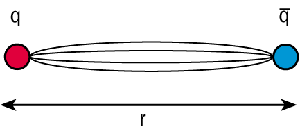
\includegraphics[scale=0.5]{Content/gluonfield.png}
 \caption{Linhas de campo entre um \emph{quark} e um \emph{antiquark}.}
 \label{linhascampo}
\end{figure}

Isso dará origem a uma densidade de energia aproximadamente constante, que dependerá
apenas da distância entre ambos:

\begin{equation}
 V(r) = -\kappa r
\end{equation}

Isso faz com que os \emph{quarks} movam-se sempre sob uma fora constante que muda de direção.
Eventualmente, na região preenchida pelo campo, devido a uma distância grande entre os \emph{quarks},
a energia do campo pode ser grande o suficiente para que um par partícula e anti-partícula se forme.
Quando isso ocorre, a energia fica distribuída em duas regiões devido a efeitos de blindagem, e teremos,
então, dois pares agora independentes, esse processo continua até que todos os pares formados não atingam
mais a distância necessária para a criação de pares. Uma descrição mais detalhada deste processo pode ser
encontrada em \cite{bierlich_rope_2017,andersson_recent_2002,skands_introduction_2013}.

%\section{Termodinâmica do QGP}\label{termo}
%Via de regra, dois observáveis estarão conectados com duas variáveis termodinâmicas referentes à matéria densa do QGP. A multiplicidade
estará conectada com a entropia, e a temperatura conectada com a energia medida. 

\section{Modelo de Glauber}\label{glauber}
Sempre que estudamos colisões de íons pesados, é necessário fornecer as condições iniciais da colisão. O modelo
de Glauber baseia-se na ideia de que os nucleons pertencentes ao núcleo projétil realizam colisões dois a dois seguindo trajetórias
retas atravessando o núcleo alvo. A distribuição dos nucleons nos dois núcleos, tanto alvo quanto o projétil, seguem a distribuição de
Woods-Saxon:

\begin{equation}
 \rho(r) = \frac{\rho_0}{1+\exp{(\frac{r-R}{a})}}
\end{equation}

Normalmente, os núcleons são gerados em uma distribuição espacial que obedece tal distribuição, em seguida, sua trajetória
é traçada em linha reta, considerando colisões com todos os núcleons em seu caminho. Uma descrição detalhada deste modelo e a
geração de condições iniciais pode ser encontrada em \cite{miller_glauber_2007}.

\end{appendices}

\bibliography{Bibliografia/bibliografia} 
\bibliographystyle{IEEEtran}
%\bibliographystyle{ieeetr}

\end{document}